\documentclass[a4paper, 14pt]{article}
\usepackage[margin=0.5in]{geometry}
\usepackage{graphicx, wrapfig} % for graphics
\usepackage{float}  % perfect fit graphic with command [H]
\usepackage{hyperref} % enable href and url
\usepackage{fullpage} % changes the margin
\usepackage{array}
\usepackage[shortlabels]{enumitem}  % to customize itemize
\usepackage[utf8]{inputenc}
\usepackage[TS1,T1]{fontenc}
\usepackage{fourier, heuristica}
\usepackage{array, booktabs}

\usepackage[x11names,table]{xcolor}
\usepackage{caption}
\DeclareCaptionFont{blue}{\color{LightSteelBlue3}}

\newcommand{\foo}{\color{LightSteelBlue3}\makebox[0pt]{\textbullet}\hskip-0.5pt\vrule width 1pt\hspace{\labelsep}}

% Set margins
\addtolength{\oddsidemargin}{-.1875in}
%\addtolength{\evensidemargin}{-.875in}
\addtolength{\textwidth}{.75in}

\addtolength{\topmargin}{-.1875in}
\addtolength{\textheight}{1.75in}

\hypersetup{
	colorlinks=true,
	linkcolor=blue,
	filecolor=magenta,      
	urlcolor=cyan,
	pdfauthor={Gahan Saraiya},
	pdfcreator={Gahan Saraiya},
	pdfproducer={Gahan Saraiya},
}

\newcolumntype{L}{>{\centering\arraybackslash}m{7cm}}
% alterante itemize command
\newcommand*\tick{\item[\Checkmark]}
\newcommand*\arrow{\item[$\Rightarrow$]}
\newcommand*\fail{\item[\XSolidBrush]}
\begin{document}
	%Header
	\begin{flushright}
		{\large \hfill \textbf{Gahan Saraiya (18MCEC10)}} \\
		\textit{
			M.Tech (CSE), Nirma University \\
			\url{gahansaraiya@gmail.com} \\
			\url{18mcec10@nirmauni.ac.in}
		}
	\end{flushright}	
	\section*{Who I Am}
	I am \href{https://www.python.org/}{\textbf{Python}} Developer since year 2015 and competent with \href{https://www.djangoproject.com/}{\textbf{Django}}, \href{http://flask.pocoo.org/}{\textbf{Flask}}, \href{https://selenium-python.readthedocs.io/}{\textbf{selenium}}.
	\\ I also like to contribute in open source too and spreading the knowledge.
	\\ Obtained Rank 112 (out of 212994)in	National Coding contest (\href{https://www.techgig.com/codegladiators}{\textbf{code gladiators 2018}}) organized by TECHGIG.
	\\ Selected for \href{https://medium.com/magentacodes/things-you-should-know-about-google-foobar-invitation-703a535bf30f}{\textbf{GOOGLE Foobar Challenge}}.
	\begin{table}[H]
		\centering
		\begin{tabular}{ L L }
			248 out of 300 score on pluralsight IQ for python. 
			& 
			{
\includegraphics[width=200px]{assets/pyIQ248.png}}
		\\ 
			\href{https://stackoverflow.com/users/flair/7664524.png}{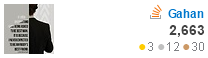
\includegraphics{assets/so7664524.png}}
			& 
			I have achieved \href{https://stackoverflow.com/users/story/7664524}{\textbf{2500+ stackoverflow}}	reputation score to guide other users in their problems
		\\ 
			\url{https://github.com/gahan9/}
			& 
			\href{https://github.com/gahan9/}{
\includegraphics[width=200px]{assets/github-logo.png}}
		\end{tabular}
	\end{table}
	
	Interested to work in Artificial Intelligence, Quantum Computing, Networking and Security, Complex Algorithms, Augmented
	Reality, Game Development.\\
	\begin{table}[H]
		\centering
		\captionsetup{font=blue, labelfont=sc, labelsep=quad}
		\caption{Academic Achievements and Extra Curriculum Activity}\vskip -1.5ex
		\renewcommand\arraystretch{1.4}\arrayrulecolor{LightSteelBlue3}
		\begin{tabular}{@{\,}r <{\hskip 2pt} !{\foo} >{\raggedright\arraybackslash}p{15cm}}
			\toprule
			\addlinespace[1.5ex]
			2017 & Runner-up in Open House’17 (State level Project Competition) for Poster Presentation \& live demo of \textbf{honeypot for network security}\\
			2016 & Zonal Winner in Cyber Security arranged by Braintech 2017\\
			2016 & Paper published in conference NCCICT 2016 (\textbf{ISBN 978-93-5288-056-0}) \\
			2015 & Catch Him If You Can - Ethical hacking workshop by Ankit Fadia (Technical Support and Organization Member) \\
			2014 - 2016 & Peer Learning Activity (Helping out Seniors, Juniors and classmates)\\
			2014 - 2018 & \textbf{Google Admin} system Administration for Institute \\
			2014 - 2016 & Technical Event and Placement Coordinator and many other volunteer activity related to technical event \\
			2014 & Configured Network boot, Ghost image for installation etc. \\
			2014 & Establishment of complete network for Department \\
			2014 & Winter Training at RTTC, Ahmedabad on \textbf{Advance Computer Network} \\
			2013-2017 & Support to Lab Assistant Faculty for setup configuration of PC/PC-health and network \\
			2014 & Server Raid-0 setup/ Raid breaking\\
			* & Fortinet Firewall (1 week) \\
		\end{tabular}
	\end{table}
	
	\newpage
	\section*{Project Detail}
	
	\begin{enumerate}[start=1,label={\bfseries $\Rightarrow$ TITLE - }]
		\addtolength{\itemindent}{40pt}
		\item SaaS for HR Management
		\\ \textbf{Duration}: November 2017 to April 2018
		\\ \textbf{Team Size}: 2
		\\ \textbf{Role Played}: Full Stack Developer
		\\ \textbf{Skills Used}: Python, Django, RESTful API development, Ajax, MySQL, SQLite, Ubuntu/Linux
		
		The system was designed to complete payment and provide a user(HR) a dashboard to manage employees, bulk upload, chat, survey creation and analytics, broadcast service
	\end{enumerate}
	
	
	\begin{enumerate}[start=1,label={\bfseries $\Rightarrow$ TITLE - }]
		\addtolength{\itemindent}{40pt}
		\item Inventory Management and GST Billing for Mobile Shop
		\\ \textbf{Duration}: May 2018
		\\ \textbf{Team Size}: 1
		\\ \textbf{Role Played}: Full Stack Developer
		\\ \textbf{Skills Used}: Python, Django, RESTful API development, Ajax, MySQL, SQLite, Ubuntu/Linux
		
		live at: \url{http://phonezilla.pythonanywhere.com}
	\end{enumerate}
	
	\begin{enumerate}[start=1,label={\bfseries $\Rightarrow$ TITLE - }]
		\addtolength{\itemindent}{40pt}
		\item Kodi Rebranding and Addon Development
		\\ \textbf{Team Size}: 2
		\\ \textbf{Role Played}: Back End Developer
		\\ \textbf{Skills used}: Python, basic C++, shell scripting, batch scripting, Kodi (v16.0 to v17.6), SQLite, Django
		
		Focused on various addon development to authenticate user by system, fetching meta data for movies and tv shows from local scattered files providing a custom Kodi build to serve content from web portal; native compilation of kodi build for android and Windows
	\end{enumerate}
	
	\begin{enumerate}[start=1,label={\bfseries $\Rightarrow$ TITLE - }]
		\addtolength{\itemindent}{40pt}
		\item Smart Interception in Network using Honeypot
		\\ \textbf{Duration}: Final Year project in B.E. (year 2016-17)
		\\ \textbf{Team Size}: 2
		\\ \textbf{Role Played}: Back End Developer
		\\ \textbf{Skills used}: Python, Django, MySQL, Ethical Hacking, Twisted
		
		available at: \url{https://github.com/Gahan9/sinh_alpha}
	\end{enumerate}

	\begin{enumerate}[start=1,label={\bfseries $\Rightarrow$ TITLE - }]
		\addtolength{\itemindent}{40pt}
		\item Surat Smart City proposal using Augmented Reality
		\\ \textbf{Duration}: year 2015
		\\ \textbf{Team Size}: 10+
		\\ \textbf{Role Played}: Research and Development
		\\ \textbf{Skills used}: basic Unity and 3ds Max, Autodesk Maya
		
		The project aimed at showcasing the future Smart City plans for Surat. Augmented Reality combined with Unity Game Engine was used to develop the walk through. The most prominent features where the models of various significant buildings and their functionalities. The project was showcased at Vibrant Gujarat 2014. The app was made for Android Platform
	\end{enumerate}
	

	\begin{enumerate}[start=1,label={\bfseries $\Rightarrow$ TITLE - }]
		\addtolength{\itemindent}{40pt}
		\item Establishment of Department Network
		\\ \textbf{Duration}: 2014 (two weeks)
		\\ \textbf{Team Size}: 20+
		\\ \textbf{Role Played}: Lead
		\\ \textbf{Skills used}:  Networking, Optimization of Cable
		
		The volunteer project lead to reestablished old network of department to fix existing network issues as well as providing connection to every user of department
	\end{enumerate}

	\newpage
	\section*{Journey to M.Tech}
	From the reading and exploring more for new technologies I always either worked or read in detail about the new technology and always eager to interact with it. \\

	At beginning I used to work on Python because of its philosophy described in \href{https://www.python.org/dev/peps/pep-0020/#the-zen-of-python}{\textbf{PEP 20 -  The Zen of Python}} and started to develop scripts for some useful. \\
	In my Bachelors study I focused more on exploring various technology and their scope and as I have explored more I came to know that I had to learn some technology or language which is near to die and replaced with various awesome technologies but more than that I learned lots of 
	When I began to explore Artificial Intelligence I came to know that the Python is best suitable language for machine learning (a Field of AI) because of it's community of packages like numpy/scipy, pandas, jupyter, sklearn etc. \\
	
	To pursue the career in research I decided to do my Masters so that I can gain more knowledge which help me build my research career. Research is not just  process which completes with just using some tools it's much more than that. I expect to gain such adequate knowledge in field of Computer Science to enhance my skills like to develop and optimize algorithm, thought spectrum.

	\section*{Life Goals}
	Inspired by various breakthrough in technology I want to pursue PhD program in  \href{http://www.mit.edu/about/}{\textbf{MIT - Massachusetts Institute of Technology}} to research in domain of Artificial Intelligence and Quantum Computing.
	
	Artificial Intelligence is the field where large dataset is analyzed and/or real time learning and decision making processed by machine. \\
%	\begin{figure}[h]
%		\centering
%		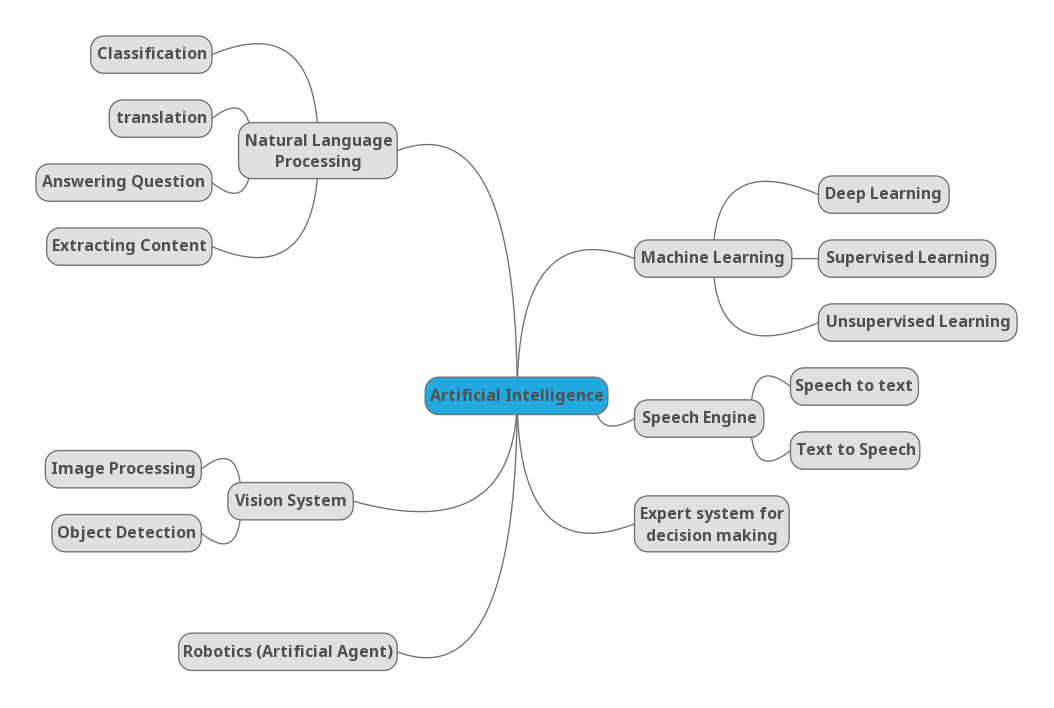
\includegraphics[scale=0.5]{assets/ai-map.png}
%		\caption{Fields of Artificial Intelligence}
%	\end{figure}
	\\
	\href{https://en.wikipedia.org/wiki/Quantum_computing}{Quantum Computing} is the future of a new programming paradigm where quantum computer performs quantum computing is built on qubits (which can be in superposition\footnote{digital system is either on state "on" or "off" but quantum computers can be on state "on" or "off" or "on and off" at the same time}) rather than binary (0 and 1). 

	\section*{Technical Skills}

	\paragraph{Languages} Python, C, CUDA, LaTeX, HTML, CSS, ajax, jquery, javascript
	\paragraph{Database} MySQL, SQLite, PostgreSQL, Blockchain
	\paragraph{Frameworks} Django, Selenium with python, Bootstrap, PyCUDA, pandas, plotly with python
	\paragraph{Tools and Technology} Git, Google Admin, PyCharm, Clion, Photoshop, MS Office, Libre Office, Prezi,
	Data Science, Web Hosting, Server Administration, Kodi Addon Development, WireShark
	
	\section*{Hobbies}
	\begin{itemize}
		\item Music
		\item Singing
		\item Chess
		\item Gaming
	\end{itemize}
%	\section*{Inspiration}
%	I believe in ideas so rather than following a single person I tend to follow ideas that drove many people to become famous in the field of research and study. I personally follow idea of "Open source" which is itself an idea followed by many communities.
%	The other quality in every successful researcher or author I have seen is patience they have great patience to get success.

\end{document}
